\begin{chapter}{Introduction to Philosophy}
    No book that mentions philosophy is complete without describing those things that are intended, or valued as goals from the book, or in corporate speak a ``vision'' for the book. This is why this book does not have a formal introduction, but finds an introduction in this section, serving to introduce the importance of formalizing goals when doing work:
        
    \begin{section}{The Intended Value of this Book}
        This is a mathematics book, and the goal of this book is to teach mathematics. However, there are many books which aim to teach mathematics, but the author feels as if there is much missing in the way of:
            
        \begin{itemize}
            \setlength{\itemsep}{6pt}
            \setlength{\parskip}{12pt}
                
            \item \textbf{Intuitions} for the concepts being taught are not commonly taught because our intuitions can often lead us astray. Oftentimes, when we teach analogies, people assume the analogies are more real than analogous, and get angry and upset when the analogies fall apart. Therefore, a long discussion must be had to explain that an analogy doesn't necessarily mean something is equivalent.
     
            \item \textbf{Examples and motivations} of the concepts being used by people. This does not mean that every example needs to be something that is used by everyone, on a daily basis. Mathematics is often argued to be independent from the physical world, and despite the truth in that, the mathematicians who discover these things are not independent of the physical world, and so the physical world still informs the mathematician, and the learner.
               
            \item Because we will focus on examples and motivation from things in the physical world, we will also add \textbf{computer programming} to our learning curriculum, building up to it, nearly from the beginning. This will be a help and a hindrance, because computer literacy and knowledge of how to set up programming environments is not a focus of the lesson plans here. In fact, we should learn what the mathematical concept of a computer is, which is not necessarily the physical thing that this book was written on, but relates to it to a very strong degree.
                
            \item Along the line of the focus on examples, we will collect \textbf{interpretations} of mathematics as it is discussed, and disseminate those interpretations as best possible.
                
            \item Furthermore, the most important thing we will do is to connect various areas of mathematics, so that intuitions from one area will carry over to the other areas, and so will the proofs. Due to this, we may prove some theorems in more than one way in this book, so that the connections can be understood, and to help demonstrate what a theorem really is.
        \end{itemize}
            
        However, the additional focus on the things listed above does not imply that this book can avoid any of the items below, and must be discussed in balance, and with sufficient detail with the following: 
            
        \begin{itemize}
            \setlength{\itemsep}{6pt}
            \setlength{\parskip}{12pt}
                
            \item Formal definitions and descriptions of the concepts, including axiomatic definitions for mathematical structures
                
            \item Various constructions of mathematical structures when possible
                
            \item Formal reasoning for the properties of mathematical structures
        \end{itemize}
            
        You'll notice that these 3 all focus on mathematical structures, which may seem like a foreign concept right now. However, we will provide some heightened understanding of what a mathematical structure is by the end of this book.
            
        The intended reader of this book is adults, and in that respect, it is andragogy (the study of teaching adults), not pedagogy (the study of teaching children). It assumes certain concepts are already understood (like an intuitive feel for the number 250, and of place-value in general); however, it is the author's opinion that the order of subject matter given in this book is approximately the best order to teach children as well, given the mathematical subject matter available as of the year 2020.
    \end{section}
        
    \begin{section}{Motivation to Learn and a Warning to Learn it Well}
        \begin{subsection}{Knowledge is One Source of Strength}
            \begin{quote}{Edward Teller}
                The science of today is the technology of tomorrow.
            \end{quote}
            
            \begin{quote}{Chinese Proverb}
                If your mind is strong, all difficult things will become easy. If your mind is weak, all easy things will become difficult.
            \end{quote}
                
            Since we are still talking about philosophy, another good argument to learn philosophy, and to learn it well, is to build a strong mind through careful analysis of: your values, your own value, what makes you strong, and how you come to understand the world around you.
                
            However, the journey through these analyses are usually very personal. The last one, ``how you come to understand the world around you'' is the only one that this book intends to address in great detail, but being a mathematical book, and not a science book, it's actually less about understanding the physical world, and more about understanding what intuitions are actually happening in your own mind.
                
            We add mathematics to this study, because we realize what it brings to our society, as far as strength goes, by giving us these glimpses into the role that our intuitions have regarding how we interpret the world around us, and how those intuitions sometimes fail, and how often they actually succeed.
                
            The role of mathematics for our society is usually at one end of the chain of information that occurs between the various STEM-based subjects:
                
            \begin{figure}[ht]
                \centering
                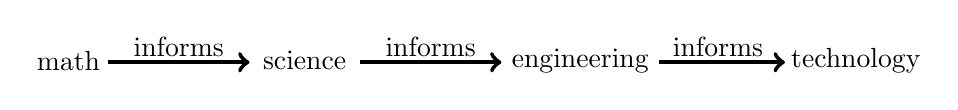
\begin{tikzpicture}
                    \node [align=center] at (0.0, 0.02){math};
                    \draw [ultra thick, ->] (0.5, 0) -- (2.3, 0);
                    \node [align=center] at (1.4, 0.2){informs};
                    \node [align=center] at (3.0, 0.02){science};
                    \draw [ultra thick, ->] (3.7, 0) -- (5.5, 0);
                    \node [align=center] at (4.6, 0.2){informs};
                    \node [align=center] at (6.5, 0.02){engineering};
                    \draw [ultra thick, ->] (7.5, 0) -- (9.1, 0);
                    \node [align=center] at (8.25, 0.2){informs};
                    \node [align=center] at (10, 0.02){technology};
                \end{tikzpicture}
            \end{figure}
                
            However, you'll also find that philosophy informs all of these, and is informed by all of these. The creative arts, like philosophy, is informed by all 4 of these, but tends towards informing only engineering and technology.
                
            This does not mean that mathematics and science is not creative, but it's often misunderstood that because mathematics is so rational, that it's not creative. It takes a lot of creative thinking and intuition, along with rational thought, in order to come up with mathematical proofs, and it is for this reason, and the connections to other fields, that creative arts is a necessary endeavour for anyone learning STEM.
                
            In fact, this is precisely the argument for STEAM.
                
            It must be stated more clearly, because the previous statement may not be clear enough: creative thinking, intuition, and rational thinking are \textbf{all} required for work in each of these fields of study, in concert with each other. Rational thinking does not promote mathematics and science alone. Intuitional thinking will almost certainly lead to falsehoods in these fields, if not matched with rational thinking.
                
            In this sense, creative thinking can be seen to be exploration, finding solution-after-solution, intuitive thinking can be seen to point the creative thinking along, but the rational thinking is the filter that finds the solutions that actually work.
                
            So, you will benefit all of these parts of your mind, including the part of you that is disciplined and builds grit. This will happen by mere practice and use, much like a muscle being used over-and-over getting bigger, and capable of handling more.
                
            Mathematics and the sciences change how you look at the world around you, but it doesn't make you a better person.
        \end{subsection}
        
        \begin{subsection}{The Danger in Strength}
            Philosophy has a long history of beneficial usage and of dangerous misuse. Philosophy may be the most important, but the most dangerous subject matter that a mind can consume. Philosophy has been used to free people as well as enslave people. The philosophical concept of moral or ethical \emph{justification} has been used both to protect and to kill.
            
            In effect, every argument about whether or not human beings are ready for a specific technology is actually a question of whether or not human beings are philosophically mature enough, and is captured in the following quotes:
            
            \begin{quote}{Jason Silva}
                Technology is, of course, a double-edged sword. Fire can cook our food but also burn us.
            \end{quote}
            
            \begin{quote}{Christian Lous Lange}
                Technology is a useful servant, but a dangerous master.
            \end{quote}
            
            \begin{quote}{B. F. Skinner}
                The real problem is not whether machines think, but whether people do.
            \end{quote}
            
            Replace ``technology'' with ``philosophy'' in the first two quotes, and you may begin to understand what it is that I'm claiming. Other quotes are a bit more direct:
            
            \begin{quote}{Martin Luther King, Jr}
                Nothing in all the world is more dangerous than sincere ignorance and conscientious stupidity.
            \end{quote}
            
            \begin{quote}{George Bernard Shaw}
                Beware false knowledge; it is more dangerous than ignorance
            \end{quote}
            
            \begin{quote}{Confucius}
                Real knowledge is to know the extent of one’s ignorance
            \end{quote}
            
            Oftentimes, it is exactly those strengths that serve as one's weaknesses, but that is not to say that having a strength necessarily creates weakness in that area. It benefits us to understand how strengths become weaknesses. 
    
            Philosophy, like technology, is good or bad, depending on how it's used, and depending on how well it's understood, and based on what principles one chooses to work from.
                
            In fact, the call-to-action I give each of you, before you start this endeavour is:
            \begin{itemize}
                \item Use your observations and experiences to help you understand your world
                    
                \item Uproot misperceptions and misunderstandings that come from a partial understanding of the first
                    
                \item Apply your understanding of the world to better your world and the world of others, as you see fit
            \end{itemize}
        \end{subsection}
        
        \begin{samepage}
            \begin{subsection}{Perceptions and Misperceptions of Philosophy, Mathematics, and Science}
                There are multiple misperceptions of about various fields of study, such as:
                \begin{itemize}
                    \item Mathematics
                    \begin{itemize}
                        \item It's not a creative field
                        \item It's the study of numbers
                        \item It's already finished (there's no new math to be had)
                        \item There are no jobs for mathematicians
                    \end{itemize}
                    
                    \item Science
                    \begin{itemize}
                        \item It's done by elite people who have no connection to reality
                        \item It's a collection of statements that are considered ``the truth''
                        \item It doesn't help ``real people''
                    \end{itemize}
                    
                    \item Software Development
                    \begin{itemize}
                        \item It's all copy-and-paste
                        \item Computers will be programming themselves soon
                        \item It's an easy desk-job with little pressure
                    \end{itemize}
                        
                    \item Economics
                    \begin{itemize}
                        \item It's the study of money
                        \item It's all psychology (which contradicts the first claim)
                    \end{itemize}
                \end{itemize}
            \end{subsection}
        \end{samepage}
            
        All of these claims are caricatures of the fields of study, or of the people who do work in those fields, and are not just oversimplifications, but are outright wrong if one were to actually follow these people around.
            
        Much the same misrepresentation occurs in all fields of study and all fields of work. These misrepresentations continue throughout the centuries as populism attempts to change the view of these subjects.
            
        The history of this populism is understood, because in history, fields such as these could only be achieved by the educated and the rich, and those people would not understand those who worked with their hands. Therefore, a schism occurred between those who used their minds, and those who used their hands, based on a classism that is not yet resolved.
            
        A shift has been occurring over the last few centuries though, especially as education has become more universal, allowing people to spend part of their lives in service, part of their lives in manual labor, part of their lives studying, and part of their lives working with their minds, and it's not certain that a person in any particular job has any particular experience.
            
        In this regard, philosophy has always been misrepresented, and you may hear things like:
        \begin{enumerate}
            \item Philosophy, like mathematics, has been completed, or it has produced all of the results and discoveries that it can
                
            \item Philosophy is useless, ungrounded, and a waste of a person's education
                
            \item Philosophy is nebulous, vague, and done by people who are out-of-touch with the real-world
                
            \item Philosophy opposes, is not supported of, or is somehow separate from science
        \end{enumerate}
            
        Nothing could be further from the truth on all of these grounds. Mathematics, and philosophy, are coming up with new discoveries all the time, and including applications to previous discoveries. Philosophy, especially the interest of how we come to know things, forms the basis for both mathematics and the sciences.
    \end{section}
    
    \begin{section}{What is Philosophy, and Why Should We Care?}
        Philosophy is typically introduced by discussing what it means, and where it comes from. We focus so much on the Greek philosophy, but philosophy, mathematics, and science has been growing in all cultures for millennia, and can be found as early trial versions of these subjects in ancient books all over the world.
            
        The word ``philosophy'' is a word from ancient Greek φιλοσοφία (\emph{philosophía}), which has 2 roots:
        \begin{itemize}
            \item φίλος (phílos meaning “loving”)
            \item σοφία (sophía meaning “wisdom”)
        \end{itemize}
            
        However, that only scratches the surface, and tends to lead to the conclusion that “philosophy is in every query”. Although this is technically true, it does little to give anyone any clue to what philosophers actually do, and why it’s important.
            
        In some ways, philosophy is the process of exploring one’s thoughts, asking ourselves, “why do I think this way?”
            
        Specifically, philosophers have certain question that all philosophy branches out from:
            
        \begin{figure}[ht]
            \centering
            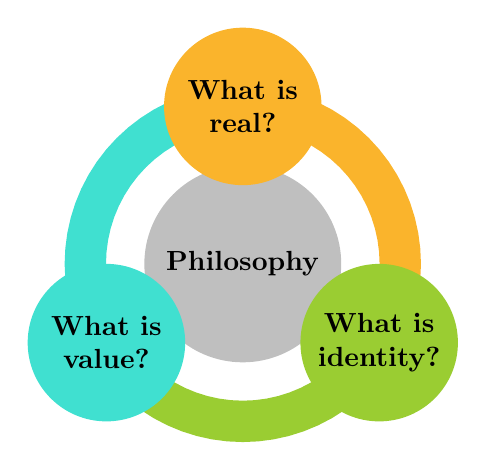
\begin{tikzpicture}
                \fill [lightgray]   (0,0) circle (12.5mm);
                \node [align=center] at (0, 0) {\textbf{Philosophy}};
                \draw [Dandelion,line width=5.25mm,domain=-30:90] plot ({2*cos(\x)},     {2*sin(\x)});
                \draw [YellowGreen,line width=5.25mm,domain=210:330] plot ({2*cos(\x)},     {2*sin(\x)});
                \draw [Turquoise,line width=5.25mm,domain=90:210] plot ({2*cos(\x)},     {2*sin(\x)});
                \fill [Dandelion] (0,2) circle (10mm);
                \fill [YellowGreen] ( 1.732,-1) circle (10mm);
                \fill [Turquoise]   (-1.732,-1) circle (10mm);
                \node [align=center] at ( 0.000, 2) {\textbf{What is}\\\textbf{real?}};
                \node [align=center] at ( 1.732,-1) {\textbf{What is}\\\textbf{identity?}};
                \node [align=center] at (-1.732,-1) {\textbf{What is}\\\textbf{value?}};
            \end{tikzpicture}
            \caption{The 3 Proposed Root Questions of Philosophy.}
            \label{fig:ThreePhilosophicalQuestions}
        \end{figure}
            
        Here though, these 3 questions feed off of each other. For instance, 
        \begin{itemize}
            \item Is it possible to seek truth without asking what methods of truth-seeking that we value?
                
            \item If something exists (if it’s “real” or “true”), can we identify it?
                
            \item If we change something (identity) does it change value?
        \end{itemize}
            
        In fact, these three questions spawn multiple branches of study, some of which are considered philosophical in modern times still, others may appear, on the surface, as if they are something separate from philosophy.
            
        \begin{subsection}{What is Real?}
            Epistemology relates to the question, “How do we know what we know?”. The study     of epistemology has given us logic (forming the foundations of mathematics),     the Scientific Method (forming the foundations of science), and gives us     mechanisms for us to understand beliefs by asking:
                
            \begin{itemize}
                \item What does it mean to know something?
                \item Can anything be known for certain? 
                \item How much confidence can we have in something?
                \item What is the process that we come to know things?
                \item What does it mean to know things?
                \item What is a belief?
                \item Can we justify our beliefs? (\textbf{critical reasoning})
                \item What is the relationship between beliefs and knowledge?     (\textbf{doxastic logic})
            \end{itemize}
        \end{subsection}
            
        \begin{subsection}{What is Identity?}
            In philosophy, we talk about \textbf{discernibility}, which lets us ask, “if two things share all the same properties, are they the same thing?”. We use this in mathematics to present two things being equal. In science, we identify phenomena that interest us. In our lives, we discuss personal identity, social identity, and even discuss the human identity. In many ways, the philosophical focus on definitions and on meanings are directly related to identifying concepts, and coming to agreement on concepts, in order to help discuss.
                
            It leads us to questions like:
                
            \begin{itemize}
                \item What does it mean for two things to be the same, and does that change over time or based on the context?
                \item If I replace every component with an identity component, is it the same thing (Interchangeability and compatibility)?
                \item Are we the same person from one moment to the next?
                \item Is any object the same from one moment to the next?
                \item How do we relate to and do we identify with our city, our culture, and/or our nation?
                \item What does it mean when things are “almost alike” or similar? And do similar things share similar properties?
            \end{itemize}
        \end{subsection}
        \begin{subsection}{What is Value?}
            The notion of \textbf{value} or \textbf{worth} is also of central concern, as it allows us to compare two things. This is also of central concern in mathematics as it allows us to make statements about relationships between things. It is of concern in modern politics, when discussing the value of citizens and whether or not they feel valued. We discuss \textbf{aesthetics} as the study of those things that attract our senses. We discuss \textbf{ethics} through the value of actions. It leads us to questions like:
                
            \begin{itemize}
                \item What does it mean to compare two things?
                \item Why do things cost what they do?
                \item What do individuals value, and why?
                \item What do societies value, and why?
                \item Is something practical worth more than something else? What makes it practical?
                \item What is fairness and justice?
            \end{itemize}
        \end{subsection}
        \begin{subsection}{What is the Relationship Between Value and Identity?}
            When questions about both value and identity come together, we usually start to ask about purpose, and
            \begin{itemize}
                \item Is there a purpose to the existence of the universe? What is the purpose?
                \item Is there a purpose to my existence? What is the purpose? Do I create my own purpose?
                \item Am I a valued part of my community? Why or why not?
                \item What is fair when it comes to treatment of different people?
                \item How does interchangeability relate to comparison? If I interchange components for something newer, is it better?
            \end{itemize}
        \end{subsection}
        \begin{subsection}{What is the Relationship Between Value and Truth?}
            This is the intersection of the two questions that lead us to asking questions like:
            \begin{itemize}
                \item How do we value the various means of obtaining knowledge?
                \item How do people value methods of communicating knowledge and beliefs?
                \item Whose testimonies do we believe and why?
                \item Can there be an absolute, top-level truth, by which all other truths are measured?
                \item Can there be a best moral code, by which all other moral codes are measured?
            \end{itemize}
        \end{subsection}
        \begin{subsection}{What is the Relationship Between Identity and Truth?}
            Regarding identity and truth, we may get some interesting questions about ourselves and:
            \begin{itemize}
                \item What are we? (i.e. what makes us human, or what makes us different?)
                \item Where do we come from?
                \item Why does anything exist at all?
                \item How do we relate to our perceptions, and vice versa?
                \item What does it mean to “exist”?
                \item What does it mean to be “real”?
                \item What is reality?
                \item What is the mind?
            \end{itemize}
        \end{subsection}
        \begin{subsection}{What is the Relationship Between All 3?}
            Finally, we can consider all 3 together:
            \begin{itemize}
                \item Is there something bigger than us?
                \item What is out there, beyond what we can perceive?
                \item How did this universe come to exist? (\textbf{cosmology})
                \item What is the greatest possible mind? Must a creator exist? (\textbf{theology})
            \end{itemize}
        \end{subsection}
            
        \begin{subsection}{Categorizing the Questions into Branches}
            Many of these questions have been placed into various categories:
            \begin{itemize}
                \item That reason can be a source of knowledge (\textbf{rationalism}) allowed us to create logic, and logic continues to refine the foundations of mathematics (classically called, “the formal sciences”)
                    
                \item Critical thinking, using our senses as a source of knowledge (\textbf{empiricism}), building confidence through experimentation (\textbf{verificationism}), and filtering in only those things that we can derive from these sources (\textbf{positivism}) refines the scientific method, which gives us science (classically called, “the physical sciences”)
                
                \item Questions about value form the basis for \textbf{Value Theory}, and include subbranches like: ethics, aesthetics, and axiology (moving into application through economics and politics)
                    
                \item Questions about existence and reality form the basis of \textbf{Metaphysics}, and include subbranches like: theology, religion, and ontology 
                    
                \item Questions about how we do philosophy form the basis of \textbf{Metaphilosophy}
            \end{itemize}
        \end{subsection}
    \end{section}
    
    \begin{section}{Philosophical Discussions}
        So, you thought that this book was going to be about mathematics. Why, then, are we learning philosophy? Well, it turns out that philosophy is the parent of almost every subject studied in any formal education. 
            
        Given that we have asked about reality, science is a formal discipline of the philosophical position called empiricism, allowing us to enter into discussion about those areas of discussion that can be observed and measured with repeatable results. However, as positions go, science is limited to such discussions.
            
        Foremost, we are interested in mathematics in this book, but we will only really get there by discussing the roots of mathematics. Also, in order to understand it, we will do best when we can also link our study to various other areas as well. The most interesting part is how these things link.
            
        \begin{figure}[ht]
            \centering
            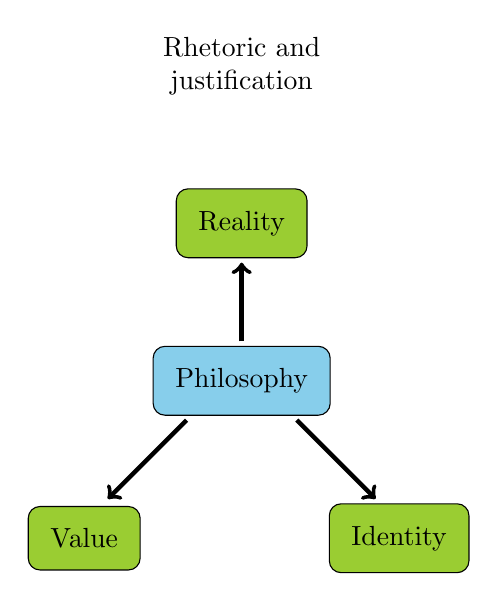
\begin{tikzpicture}
                \node [align=center,draw=black,fill=SkyBlue,thin,inner sep=8pt,rounded corners=.15cm] at (0.0, 0.0) {Philosophy};
                
                \node [align=center,draw=black,fill=YellowGreen,thin,inner sep=8pt,rounded corners=.15cm] at (0.0, 2.0) {Reality};
                
                \node [align=center] at (0.0, 4.0) {Rhetoric and\\justification};
                
                \node [align=center,draw=black,fill=YellowGreen,thin,inner sep=8pt,rounded corners=.15cm] at (-2, -2.0) {Value};
                
                \node [align=center,draw=black,fill=YellowGreen,thin,inner sep=8pt,rounded corners=.15cm] at ( 2, -2.0) {Identity};
                
                \draw [ultra thick, ->] ( 0.0, 0.5) -- (0.0, 1.5);
                \draw [ultra thick, ->] (-0.7,-0.5) -- (-1.7, -1.5);
                \draw [ultra thick, ->] ( 0.7,-0.5) -- ( 1.7, -1.5);
                %\node [align=center] at (0.0, 0.02){math};
                %\draw [ultra thick, ->] (0.5, 0) -- (2.3, 0);
                %\node [align=center] at (1.4, 0.2){informs};
                %\node [align=center] at (3.0, 0.02){science};
                %\draw [ultra thick, ->] (3.7, 0) -- (5.5, 0);
                %\node [align=center] at (4.6, 0.2){informs};
                %\node [align=center] at (6.5, 0.02){engineering};
                %\draw [ultra thick, ->] (7.5, 0) -- (9.1, 0);
                %%\node [align=center] at (8.25, 0.2){informs};
                %\node [align=center] at (10, 0.02){technology};
            \end{tikzpicture}
        \end{figure}
            
        \begin{figure}[H]
            \centering
            \includegraphics[scale=0.65]{PhilosophicalIntroduction/ConnectionsToPhilosophy.png}
            \caption{Connections of Various Fields to Philosophy.}
            \label{fig:ConnectionsToPhilosophy}
        \end{figure}
            
        \begin{subsection}{Rhetoric and Justifying Beliefs}
            It's important to understand that much of our mental sophistication revolves around explaining ourselves to others, whether that be in regards to giving them a mental image of what we have seen, explaining how something works, to justifying our reasons for doing something.
                
            Jonathan Haidt gave us the analogy of our minds being of a human rider on top of an elephant, whereas the rider is the rational mind, and the intuition is the elephant. We are so good at justifying our actions to others, that we often justify things we have done to ourselves, even when we know better (e.g. ``I can eat that whole chocolate cake, because I've done so well on my diet this week.'').
                
            Our written Greek philosophy seems to start with regards to \textbf{rhetoric}, as the ``art of discussion'', developing the communication skills to discuss philosophical positions.
                
            Rhetoric was often divided into:
            \begin{itemize}
                \item \textbf{Emotional} appeals, intended to speak directly to the mind's elephant. These appeals are often highly effective, if sometimes manipulative in their usage.
                    
                \item \textbf{Authoritative} appeals, intended to invoke the authority of the speaker, through their experience or due to their character-history of truthfulness.
                    
                \item \textbf{Rational} appeals, intended to speak directly to the rider of the elephant, who is capable of mapping out a direction for the elephant to travel, if the rider can ever get the elephant to listen.
            \end{itemize}
                
            We may be used to hearing the word rhetoric in political discussions (such as ``inflammatory rhetoric''), but oftentimes the person using the word doesn't mean it with the nuance of the philosophical meaning. Instead, philosophers would deem what politicians are doing \textbf{polemic}, which is emotional arguments intended to reduce confidence in and incite fear of an opponent.
                
            It should be obvious that mathematics and the sciences are filled with logical appeals, and as such, this book will be filled with them as well. However, it's also recognized that the intuition must be brought on board as well. 
                
            Finally, the authoritative appeals should be mostly unused in any discussion of mathematics. There is no for a teacher to use appeals to authority, saying things like ``it just works this way''. The only authoritative appeals will be the usage of already defined and commonly used standards for writing that may be brought up. However, even those should be backed with arguments for rational reasons why.
                
            \begin{subsubsection}{Some Definitions}
                
                \begin{definition}
                    An \textbf{interlocutor} is a person that is taking part in a dialog.
                \end{definition}
                    
                \begin{definition}
                    A \textbf{proposition} is a statement is possibly true or false.
                \end{definition}
                    
                \begin{definition}
                    A \textbf{premise} is a proposition for consideration, sometimes asserted as true by the interlocutor, and sometimes as a condition for the context of the argument.
                \end{definition}
                    
                \begin{definition}
                    A \textbf{conclusion} is a proposition that is the end result that the interlocutor reaches starting from the premises.
                \end{definition}
                    
                \begin{definition}
                    An \textbf{argument} is a series of propositions, structured such that the premises lead to a conclusion. Furthermore, a more general meaning of this word may be a process of reasoning.
                \end{definition}
                    
                \begin{definition}
                    A premise taken as a condition, usually in regards to an investigation is called a \textbf{hypothesis}.
                \end{definition}
                    
                \begin{definition}
                    A \textbf{philosophical position} is a collection of premises that an interlocutor is arguing from.
                        
                    It is often called a \textbf{philosophical theory}, which can cause confusion with the significantly different meanings taken by scientific theory and mathematical theory. 
                        
                    The everyday usage of the word ``theory'' is probably best identified as ``hypothesis''.
                        
                    Due to this confusion, the word position will be preferred in this book.
                \end{definition}
                    
                \begin{figure}[ht]
                    \centering
                    
\begin{tikzpicture}
                        \node [align=right] at (0.0, 0.02){position};
                        \draw [ultra thick, ->] (0.7, 0) -- (2.3, 0);
                        \node [align=center] at (1.4, 0.2){argument};
                        \node [align=left] at (3.2, 0.02){conclusion};
                    \end{tikzpicture}
                    \caption{Relation between position (premises), argument, and conclusion}
                \end{figure}
                    
                \begin{definition}
                    For the sake of comparison, a \textbf{life stance} is a philosophical position that one takes, according to their worldview, which informs their beliefs, their thoughts, and their behavior.
                        
                    This is stated separately, since a life stance differs from a philosophical position.
                \end{definition}
                    
                \begin{definition}
                    A \textbf{Devil's Advocate} is a person that argues from a position that differs from their life stance, in order to better understand their own position, and the position of others.
                \end{definition}
                    
                \begin{definition}
                    \textbf{Skepticism} is the act of reserving belief for future evidence.
                \end{definition}
                
                \begin{definition}
                    \textbf{Belief revision} is the act of modifying one or more premises that make up a position, due to new evidence.
                \end{definition}
            \end{subsubsection}
            
            \begin{subsubsection}{What Forms a Worldview}
                At this point, I'm going to present what follows as a position, setting the rest of the book up for discussions on logical reasoning.
                    
                \begin{remark}
                    This position I am starting from, regarding worldviews, is not scientific, is not based on psychological evidence, and is likely just an approximation of how worldviews actually work.
                \end{remark}
                    
                \begin{figure}[ht]
                    \centering
                    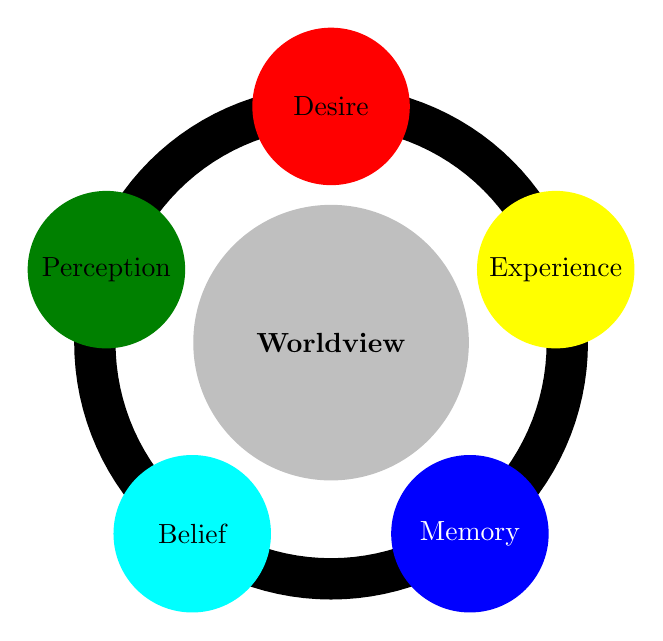
\begin{tikzpicture}
                        \fill [lightgray] (0,0) circle (1.75cm);
                        \node [align=center] at (0, 0) {\textbf{Worldview}};
                            
                        \draw [Black,line width=5.25mm,domain=90:162] plot ({3*cos(\x)}, {3*sin(\x)});
                        \draw [Black,line width=5.25mm,domain=162:234] plot ({3*cos(\x)}, {3*sin(\x)});
                        \draw [Black,line width=5.25mm,domain=234:306] plot ({3*cos(\x)}, {3*sin(\x)});
                        \draw [Black,line width=5.25mm,domain=306:378] plot ({3*cos(\x)}, {3*sin(\x)});
                        \draw [Black,line width=5.25mm,domain=378:450] plot ({3*cos(\x)}, {3*sin(\x)});
                            
                        \fill [Red]   ( 0.000000, 3.000000) circle (10mm);
                        \fill [Green] (-2.853170, 0.927051) circle (10mm);
                        \fill [Cyan]  (-1.763356,-2.427051) circle (10mm);
                        \fill [Blue]  ( 1.763356,-2.427051) circle (10mm);
                        \fill [Yellow]( 2.853170, 0.927051) circle (10mm);
                            
                        \node [align=center,text=black] at 
                        ( 0.000000, 3.000000) {Desire};
                        \node [align=center,text=black] at 
                        (-2.853170, 0.927051) {Perception};
                        \node [align=center,text=black] at 
                        (-1.763356,-2.427051) {Belief};
                        \node [align=center,text=white] at 
                        ( 1.763356,-2.427051) {Memory};
                        \node [align=center,text=black] at 
                        ( 2.853170, 0.927051) {Experience};
                    \end{tikzpicture}
                    \caption{Relation between position (premises), argument, and conclusion}
                \end{figure}
                    
                The first question someone may have looking at the components of a person's worldview that I listed is that experience, memory, and belief are all the same thing. However, my argument is that we experience all the time, but our beliefs color how we interpret the memories associated with those experiences.
                    
                In this sense, we reexperience things through our memory, but it doesn't mean that it feels the same each time.
                    
                It may seem strange that I put desire in with the rest of these, because it appears that the rest of these relate to knowledge, but that desire is completely unrelated. However, we already know that desires change how we perceive things, making us more or less perceptive of our failures or successes, or how other people act.
                    
                The point of all of this is to say that our memories are fallible, because they change. Our perceptions are fallible as well, and so, we cannot always trust our worldview.
            \end{subsubsection}
                
            \begin{subsubsection}{What Sources of Information do you Value?}
                In the discussion of rhetoric, we talked about 3 different types of arguments: emotional, authoritative, and rational.
                    
                However, these are only the methods of transference of information from one person to another, and misses an important source of information: experience.
                    
                We tend to regard experience as the most valued source of information, but as we discussed in regards to the worldview, our perceptions of experiences are often incomplete, and sometimes even wrong.
                    
                Most people, naturally value emotional, authoritative, experiential, intuitive, and rational information sources to some level or another, because we naturally recognize that there are failings with putting all of our trust in any one of them: emotions can sometimes be erratic, people sometimes lie, our perceptions often deceive us, our intuitions are often wrong, and we often don't have enough information to come to a rational conclusion.
                    
                However, there are things that we can do to refine when we use each, and what we can be said about each source of information.
                    
                Firstly, it's important to note that rational arguments begin as intuitive arguments. Humans have an intuitive ability to recognize cause-and-effect, allowing us to determine how things work, and often change how things work to our favor. This recognition of the pattern of cause-and-effect is what leads us to logic, and rational thinking is the disciplined use of this logic. 
                    
                In fact, the discipline is what separates intuition from rational thinking. We follow through with our intuitions to see if they fail.
                    
                Second, the relationship between emotions and intuition are also important. Purely rational thinking is devoid of creativity, can get stuck in analysis, and therefore absent problem solving ability. However, purely intuitive thinking cannot weed out those ideas that won't work, and will naturally try things that are not logically sound, usually wasting their own and other people's time.
                    
                First, let's get more detailed how these each operate as a source of information:
                \begin{itemize}
                        
                    \item Authoritative sources
                    \begin{itemize}
                        \item \textbf{Witnesses} can provide accounts of events
                        \item Parents and teachers often provide us tons of information
                    \end{itemize}
                    \item Experiential sources
                    \begin{itemize}
                        \item Your \textbf{senses} give you access to the world around you and are your connection to it
                        \item When your senses act together they create an \textbf{empirical} view of the world
                        \item This effectively places you as an authority over your own worldview
                        \item Demonstrations from other individuals can help communicate subject matter
                    \end{itemize}
                    \item Emotional and Intuitive sources
                    \begin{itemize}
                        \item Emotions can point us to how our intuitions react to specific experiences
                        \item Gut feelings can tell us things about our world, and are frequently part of our mental pattern-matching capabilities.
                        \item It is via these gut feelings that we are capable of walking, knowing where to place each foot as we move
                        \item The intuitive is unconscious, but quick to form conclusions
                    \end{itemize}
                    \item Rational sources
                    \begin{itemize}
                        \item We use logic and probability to determine whether or not something is possible
                        \item We use analogy to compare and contrast things that we know against things that we do not know
                    \end{itemize}
                \end{itemize}
                    
                We know that authorities can lie, and that witnesses can't always trust their memories. Likewise, we cannot always trust our senses, nor our memories. Our emotions and intuitions are often wrong. Also, we can misuse logic, probability, and analogy.
                    
                In seeking information that we can trust, it seems like we are out of luck, but through careful inspection, we can begin to clear out the mess.
                        
                Regarding rational and intuitive thought, if we learn how to properly use logic and to understand our own biases, we can balance intuition with rational thinking, by allowing intuition to come up with hypotheses, and cutting through the wrong ones via rational thought. We can learn how where rational thinking works, and how sometimes fails us.
                    
                Regarding experience, we can learn about our own psychology, and also through our biases, determine when we can trust our senses and our experiences. We can determine whether multiple memories working together with evidence can corroborate our hypotheses.
                    
                Regarding authorities, \textbf{Subject Matter Experts} are people who are experienced in a subject matter and have a record of insightful discussions, and as long as they have no motive to lie to us, information inside their area of expertise can be trusted.
                    
                From there, we can actually learn what authorities know, how they came to their conclusions, and come to conclusions ourselves via experience and rational thinking.
                    
                So, it's important to think about how and why you value the sources of information that you do, how and why they can fail you, and how to effectively work through them.
            \end{subsubsection}
                
            \begin{subsubsection}{Epistemology}
                The study of what we know and how we come to know it is called \textbf{epistemology}. It is extremely important in the realm of mathematics and the sciences to understand epistemology, 
            \end{subsubsection}
            \begin{subsubsection}{Rigorous Communication}
                Furthermore, most of this communication between experts requires that the words they use are well-understood. We have definitions for words that we use all the time, but often words in a particular \emph{subject matter} have explicit definitions which differ from how they are used in everyday speech.
                    
                Let's consider one of the most problematic words in use today. The word \textbf{theory} from the ancient Greek θεωρία (``theoria'') was contrasted to πρᾶξις (``praxis'' where we get the word ``practice''). The theory behind something was the contemplation regarding how an activity works, and the praxis was the act of doing it. Therefore, theory was used to improve the praxis, but praxis was used to improve the theory.
                    
                This contrasting terminology between the two is why we still have phrases like ``that's works in theory, but not in practice''. However, the meaning of theory in our everyday life is not necessarily how it is used elsewhere:
                    
                \begin{itemize}
                    \item \textbf{Theory (science)} -- a hypothesis which is confirmed by repeated and thorough experimental observation to provide reliable predictions
                    
                    \item \textbf{Theory (mathematics)} -- the collection of premises and conclusions related specific mathematical structures
                        
                    \item \textbf{Theory (philosophy)} -- the collections of premises and conclusions specific to an area of philosophical pursuit (also called a philosophical position).
                        
                    \item \textbf{Theory (everyday speech)} -- a proposed explanation serving as a hypothesis
                \end{itemize}
            \end{subsubsection}
                
                
        \end{subsection}
        \begin{subsection}{Ontology and the Mathematics of Identity, Equality, and Equivalence}
            Discernibility
            Distinguisibility
            Interchangeability
            Identical
                
            \begin{subsubsection}{Definitions}
                In every field of study, we have to be extremely careful what it is we mean when we say something, and aim to avoid
                    
                In mathematics, we often define something, to use in a context (a scope of discussion) and when we are done, we stop meaning it the same. In speech, we do this often with pronouns. For instance, ``Caleb left work. He wasn't feeling that well.''. We immediately know that `He' in the sentence refers to Caleb. In this case, with English, we didn't even specifically define that we'd use `He' this way.
            \end{subsubsection}
                
                
            \begin{subsubsection}{Isomorphisms}
                \begin{definition}
                    The word \textbf{isomorphism} has a formal definition that we will cover later in Category Theory. Philosophically, it can be thought best to first recognize that mathematical objects are conceptual, not physical, and we can argue only that two objects constructed exactly the same way (structural identity) are identical. However, as we have said, two objects can be constructed in 2 different ways and behave as if they are the same object. These objects then have interchangeability between them.
                    
                    An isomorphism focuses, not on identical constructions (what the objects ``are''), but on identical behaviors (what the objects ``do''), and more specifically, that they adhere to the same ``legal contracts'' we call axioms.
                    
                    The word isomorphism (iso- ``same'', -morphism ``form'') is an effective ``equality between types of things''. 
                \end{definition}
                
                An example would be the 2 identical definitions for the number 1:
                \begin{enumerate}
                    \item The natural number comes after 0
                    \item The unique natural number that allows us to multiply any number by itself and result in the same number
                \end{enumerate}
                
                Both of those definitions for 1 focus on what it does, but the first definition is closer to the actual construction of 1 than the second. The two definitions are isomorphic to each other.
                    
                Furthermore, we have the Univalence Axiom, which binds multiple mathematical fields together, in the same way that René Descartés bound algebra together with geometry when he noticed that we can put things on a grid. The proposal of the Univalence Axiom first observed that equivalence (structural identity) implies isomorphism(interchangeability), but the true observation was that an isomorphism was interchangeable with an equivalence.
                
                Now, that's not being fully honest, and yet it is at the same time. A good philosopher will think to themselves, ``you didn't use the word `equivalence' the same way in both of those sentences'', and that philosopher would be right.
                
                I started the discussion talking about identical constructions (what objects ``are''),and obviously, two things cannot be equivalent if they do not have identical constructions. However, equivalence doesn't have to mean identical constructions.Mathematicians often define equivalence based on interchangeability in the same sense as the following analogy:
                
                \begin{quote}
                    A ``Gizmo'' machine has a component called a ``doohickey''. If I can take the doohickey out and replace it with another doohickey, they are interchangeable. If I can replace the Gizmo with another Gizmo, and use the same doohickey in both, then the Gizmo itself is fungible (interchangeable with other things that use components). If any doohickey can go in any Gizmo, then the differences between each doohickey is indiscernible.
                \end{quote}
                
                So, we get an isomorphism between algebraic equations and geometry from Descartés. From Euler we'll see how trigonometry, calculus, and complex numbers relate. However, here we use this opportunity to note that there is an isomorphism between paths, logic,partial orders, computation (and computer science), and tons of things we may get to later, just from Vladimir Voevodsky's Univalence Axiom.
                
                Finally, I have mentioned Axioms as ``legal contracts for mathematical structures''.You may be asking, what structure do we assume Univalence for? We will eventually get into Category Theory, and that will help combine all the world of mathematics together for us.
                
                So, it helps to understand that equality has context, just as isomorphism has context, and we may discuss various types of equalities.
            \end{subsubsection}
                
            \begin{subsubsection}{Natural Numbers are not Non-negative Integers}
                Never does the distinction and non-distinction matter as much as how we teach the number classifications. We have probably been taught that we can identify integers as allowing for negative numbers, and that every natural numbers \textbf{is} an integer.
                    
                This notion of \textbf{is} refers to our isomorphism from earlier. We can construct integers, and we can construct natural numbers, and we will construct them later, but the statement ``\textbf{is}'' used above must be understood to mean that we can get an integer from a natural number, and take that same integer and find a natural number that matches it. That is what it means to ``be the same''.
            \end{subsubsection}
        \end{subsection}
    \end{section}
\end{chapter}